\section{Another way to look at knot colorings}

Alexander in his work colored the regions of a knot diagram as he related the resulting knot invariant to the Dehn presentation of the knot group \cite{alex-oryginal}. Today we know about the Wirtinger presentation to which coloring of arcs of a diagram can be related.

\begin{definition}[Wirtinger presentation]
  Take $D$ to be an oriented diagram of knot $K$ with $n$ segments $s_1,..., s_n$ and $n$ crossings $x_1,...,x_n$. The fundamental group of $K$ has the following presentation
  $$\pi_1(S^3-K)=\langle s_1,..., s_n\;|\;x_1,...,x_n\rangle,$$
  where each crossing $x_i$ represents one of the following relations, depending on its type

  \begin{center}
    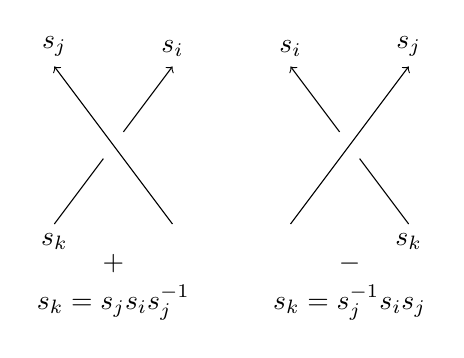
\begin{tikzpicture}
      \draw[->] (0,0) node[below] {$s_k$} -- (1.5, 2) node[above] {$s_i$};
      \fill[white] (0.75, 1) circle (6pt);
      \draw[->] (1.5, 0)--(0, 2) node[above] {$s_j$};
      \node at (0.75, -0.5) {$+$};
      \node at (0.75, -1) {$s_k=s_j s_i s_j^{-1}$};

      \draw[->] (4.5, 0) node[below] {$s_k$} --(3, 2) node[above] {$s_i$};
      \fill[white] (3.75, 1) circle (6pt);
      \draw[->] (3, 0)--(4.5, 2) node[above] {$s_j$};
      \node at (3.75, -0.5) {$-$};
      \node at (3.75, -1) {$s_k=s_j^{-1} s_i s_j$};
    \end{tikzpicture}
  \end{center}
\end{definition}

Take $G=\pi_1(S^3-K)$. Using the Mayer-Vietoris sequence we can show that $G^{ab}=\Z$ regardless of the structure of $K$. Thus we need to work more carefully with $G$ to obtain a reasonable invariant. Consider the following two exact sequences
\begin{center}
  \begin{tikzcd}
    0\arrow[r] & K=[G, G]\arrow[r]\arrow[d] & G\arrow[r]\arrow[d] & \Z \arrow[r]\arrow[d, "id" right] & 0 \\ 
    0 \arrow[r] & K^{ab} \arrow[r] & G^{mab} \arrow[r] & \Z \arrow[r] & 0
  \end{tikzcd}
\end{center}
where both arrows $K\to K^{ab}$ and $G\to G^{mab}$ are quotient maps of $[K, K]$.

\begin{lemma}\label{jadro abeliazniacji}
  Let $s_1,..., s_n$ be the generating set of $G$ and take $a_i=s_is_1^{-1}$ for $i=2,...,n$ and $a_1=s_1$ to be the new generating set. Then $K$ is generated by $s_1^{k}a_is_1^{-k}$ for $k\in\Z$ and $i=2,...,n$.
\end{lemma}

\begin{proof}
  {\large\color{red}TODO}
\end{proof}

Thanks to \cref{jadro abeliazniacji} we can now define the structure of $\Z[\Z]$ module on $K^{ab}$ by
$$t(a_i)=s_1a_is_1^{-1}$$
for $i=2,...,n$. From now on we will think of $K^{ab}$ as a $\Z[\Z]$-module.

\begin{definition}[Alexander matrix]
  Let $G$ be the fundamental group of a knot $K$. Consider the following resolution of $\Z[\Z]$-module $K^{ab}$
  \begin{center}
    \begin{tikzcd}
      ...\arrow[r] & \Z[\Z]^a\arrow[r, "A_D"] & \Z[\Z]^b\arrow[r] & K^{ab}\arrow[r] & 0
    \end{tikzcd}
  \end{center}
  The matrix associated with homomorphism $A_D$ is called the \buff{Alexander matrix} of $G$.
\end{definition}

When $G$ has the Wirtinger presentation with $n$ generators, then $K^{ab}$ has resolution 
\begin{center}
  \begin{tikzcd}
    0\arrow[r] & \Z[\Z] \arrow[r] & \Z[\Z]^{n-1} \arrow[r, "A_D"] & \Z[\Z]^n \arrow[r] & K^{ab} \arrow[r] & 0
  \end{tikzcd}
\end{center}








